\documentclass[10pt, a4paper]{article}
\usepackage{preamble}
\usepackage{calc}

\title{Discrete Mathematics}
\author{}
\date{January 2025}

\begin{document}

\maketitle

\newpage

\section{Flows and Matchings}

\begin{definition}
    Let $V$ be a finite set,
    the vertices,
    containing two special
    (distinct)
    elements $s$
    (the source)
    and $t$
    (the sink).
    Suppose for every ordered pair $u, v \in V$ we have a capacity $c_{uv}$,
    which is a non-negative integer;
    denote the set of capacities by $C = \{c_{uv}\,:\,u, v \in V\}$.
    We call $(V, C)$ a capacitated network.
\end{definition}

If we have some resource we want to move from the source $s$ to the sink $t$.
We have unlimited resource to transport,
we are limited by the fact that we must route the resource from vertex to vertex is bounded by the capacity $c_{uv}$.
If $c_{uv} = 0$,
we cannot move anything directly from $u$ to $v$,
however there may be an indirect route.

\textbf{Application examples}:

Water flows through pipes,
or a river network,
linking the vertices of $V$.
Our capacity of the river or pipe is the volume of water which can pass through per unit time.

In a road network built on the cities located at vertices of $V$,
traffic can get from city $s$ to city $t$.
The capacity of the road would be how many cars can travel the route per unit time.


We should look at directed graph.

\begin{definition}
    Given a capacitated network $(V, C)$,
    let $E$ be the set of directed edges $E = \{(u, v)\,:\, u, v \in V, c_{uv} > 0\}$.
    Then $G = (V, E)$ is the directed graph representing the available routes on vertices $V$ given capacities $C$.
\end{definition}

Usually we write $uv$ for $(u, v)$.

For convenience,
we will assume:
\begin{enumerate}[label = (\roman*)]
    \item our directed graph has no loops,
    meaning that we suppose that $c_{uu} = 0$ for all $u \in V$;

    \item there's a directed path from $s$ to $t$,
    meaning a sequence of vertices $v_0, \dotsc, v_k \in V$ such that $s = v_0$,
    $t = v_k$,
    $v_{i - 1}v_i \in E$ and for each $1 \leq i \leq k$.
\end{enumerate}

\begin{definition}
    A flow $F$ over the network $(V, C)$ is a set of non-negative integers,
    the flow values,
    $F = \{f_{uv}\,:\, u, v \in V\}$,
    satisfying:
    \begin{enumerate}[label = (\roman*)]
        \item for all $u, v \in V$,
        one has $f_{uv} \leq c_{uv}$,
        i.e.,
        the flow along a directed edge cannot exceed its capacity;

        \item at each vertex $v$ other than $s$ or $t$,
        the sum of the flow values on edges arriving at $v$ is equal to the sum of the flow values on edges leaving $v$.
    \end{enumerate}
\end{definition}


\begin{example}
    Explain why the second condition in the definition of a flow can be expressed as
    \[
    \sum_{u \in V}f_{uv} - \sum_{u \in V}f_{vu} = 0,\qquad\text{provided $v \notin \{s, t\}$}.
    \]
    What if $v = s$ or $t$?
    Define $\Phi_{in}(F) = \sum_{v \in V}f_{sv} - \sum_{u \in V}f_{us}$
    (the net amount of flow generated by the source)
    and $\Phi_{out}(F) = \sum_{u \in V}f_{ut} - \sum_{v \in V}f_{tv}$
    (the net amount of flow drained at the sink).
    
    \begin{solution}
        We have $V = \{v_1, \dotsc, v_N\}$
        (\textit{Note:
        we are including the source $s$ and sink $t$ in the set of vertices $V$})
        \[
        \sum_{u \in V}f_{uv} - \sum_{u \in V}f_{vu} = 0
        \]
        \[
        \sum_{u \in V}f_{uv}  = f_{v_1v} + f_{v_2v} + \dotsc + f_{v_nv} = \text{the flow into $v$}
        \]
        \[
        \sum_{u \in V}f_{vu}  = f_{vv_1} + f_{vv_2} + \dotsc + f_{vv_n} = \text{the flow out of $v$}.
        \]
        So the flow into $v$ equals the flow out of $v$.
    \end{solution}
\end{example}

\begin{example}
    Explain why $\sum_{u, v \in V}f_{uv} = \sum_{u, v \in V}f_{vu}$
    (this uses neither of the properties of a flow).
    Use this together with the formula in the previous exercise to show that $\Phi_{in}(F) = \Phi_{out}(F)$.

    \begin{solution}
        By the cases $u, v \in V \setminus \{s, t\}$.
        We can apply the previous repeatedly for any $v \in V \setminus \{s, t\}$.

        Now for $u, v \in \{s, t\}$.
        Flow into $s$ is $0$,
        $f_{vs} = 0$ for all $v \in V$ because there are no loops and the source only goes out.
        $\sum_{v \in V}f_{sv} = \sum_{v \in V}f_{vt}$
        (the flow out of $s$ to $v$ is equal to the flow from $v$ to $t$)
        because the flow into any vertex equals the flow going out of any vertex.
        $f_{tv} = 0$ for all $v \in V$ since there's no flow going out of $t$.
    \end{solution}
\end{example}

\begin{definition}
    We call $\Phi_{tot}(F) := \Phi_{in}(F) = \Phi_{out}(F)$ the total value of the flow $F$.
\end{definition}

\begin{example}
    What are the values of $\Phi_{tot}$ for the two flows in the following graph.
    Can you find a flow with a greater value of $\Phi_{tot}$?
    What is the best you can do?

    \begin{figure}[H]
        \centering
            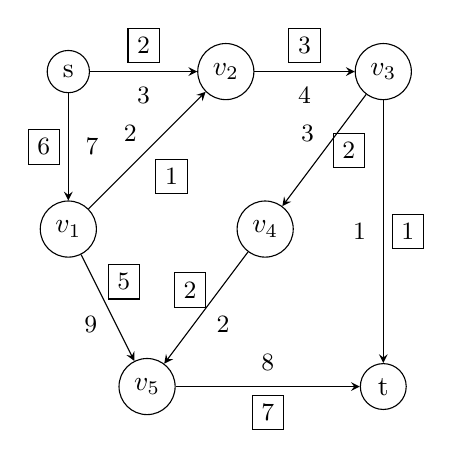
\begin{tikzpicture}[>=stealth, node distance=2cm, every node/.style={draw, circle}]
                % Nodes
                \node[draw] at (0, 0) (s) {s};
                \node[draw] at (0, -2) (v1) {$v_1$};
                \node[draw] at (2, 0) (v2) {$v_2$};
                \node[draw] at (4, 0) (v3) {$v_3$};
                \node[draw] at (2.5, -2) (v4) {$v_4$};
                \node[draw] at (1, -4) (v5) {$v_5$};
                \node[draw] at (4, -4) (t) {t};
        
                % Edges
                \draw[->] (s) -- (v2)
                    node[midway, above, rectangle, yshift = 3pt] {\small 2} 
                    node[midway, below, draw = none] {\small 3};
                    
                \draw[->] (s) -- (v1)
                    node[midway, left, xshift = -3pt, rectangle] {\small 6}
                    node[midway, right, draw = none] {\small 7};
                    
                \draw[->] (v1) -- (v2)
                    node[midway, below right, rectangle, xshift = 3pt, yshift = -3pt] {\small 1}
                    node[midway, above left, draw = none] {\small 2};
                    
                \draw[->] (v1) -- (v5)
                    node[midway, above right, rectangle, yshift = 3pt] {\small 5}
                    node[midway, below left, draw = none] {\small 9};
                
                \draw[->] (v2) -- (v3)
                    node[midway, above, rectangle, yshift = 3pt] {\small 3}
                    node[midway, below, draw = none] {\small 4};
                
                \draw[->] (v3) -- (t)
                    node[midway, right, rectangle, xshift = 3pt] {\small 1}
                    node[midway, left, draw = none] {\small 1};
                
                \draw[->] (v3) -- (v4)
                    node[midway, right, rectangle, xshift = 3pt] {\small 2}
                    node[midway, above left, draw = none] {\small 3};
                
                \draw[->] (v4) -- (v5)
                    node[midway, above left, rectangle] {\small 2}
                    node[midway, below right, draw = none] {\small 2};
                
                \draw[->] (v5) -- (t)
                    node[midway, below, rectangle, yshift = -3pt] {\small 7}
                    node[midway, above, draw = none] {\small 8};
            \end{tikzpicture}
            
            \begin{solution}
                We can see that the best $\Phi_{tot}(F)$ will be $8$ as we can increase the flow along the edge $sv_1$,
                $v_1v_5$ and $v_5t$ to get them to their capacities or closer to,
                e.g.
    
                \begin{figure}[H]
                    \centering
                    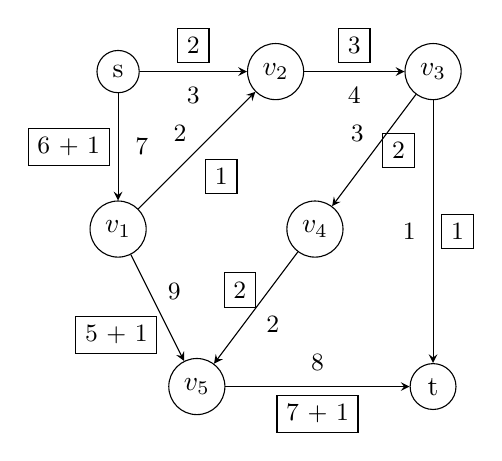
\begin{tikzpicture}[>=stealth, node distance=2cm, every node/.style={draw, circle}]
                        % Nodes
                        \node[draw] at (0, 0) (s) {s};
                        \node[draw] at (0, -2) (v1) {$v_1$};
                        \node[draw] at (2, 0) (v2) {$v_2$};
                        \node[draw] at (4, 0) (v3) {$v_3$};
                        \node[draw] at (2.5, -2) (v4) {$v_4$};
                        \node[draw] at (1, -4) (v5) {$v_5$};
                        \node[draw] at (4, -4) (t) {t};
                
                        % Edges
                        \draw[->] (s) -- (v2)
                            node[midway, above, rectangle, yshift = 3pt] {\small 2} 
                            node[midway, below, draw = none] {\small 3};
                            
                        \draw[->] (s) -- (v1)
                            node[midway, left, xshift = -3pt, rectangle] {\small 6 + 1}
                            node[midway, right, draw = none] {\small 7};
                            
                        \draw[->] (v1) -- (v2)
                            node[midway, below right, rectangle, xshift = 3pt, yshift = -3pt] {\small 1}
                            node[midway, above left, draw = none] {\small 2};
                            
                        \draw[->] (v1) -- (v5)
                            node[midway, below left, rectangle, yshift = -3pt] {\small 5 + 1}
                            node[midway, above right, draw = none] {\small 9};
                        
                        \draw[->] (v2) -- (v3)
                            node[midway, above, rectangle, yshift = 3pt] {\small 3}
                            node[midway, below, draw = none] {\small 4};
                        
                        \draw[->] (v3) -- (t)
                            node[midway, right, rectangle, xshift = 3pt] {\small 1}
                            node[midway, left, draw = none] {\small 1};
                        
                        \draw[->] (v3) -- (v4)
                            node[midway, right, rectangle, xshift = 3pt] {\small 2}
                            node[midway, above left, draw = none] {\small 3};
                        
                        \draw[->] (v4) -- (v5)
                            node[midway, above left, rectangle] {\small 2}
                            node[midway, below right, draw = none] {\small 2};
                        
                        \draw[->] (v5) -- (t)
                            node[midway, below, rectangle, yshift = -3pt] {\small 7 + 1}
                            node[midway, above, draw = none] {\small 8};
                    \end{tikzpicture}
                \end{figure}
        \end{solution}
    \end{figure}
\end{example}

\begin{definition}
    Let $S \subset V$ with $s \in S$ and $t \notin S$.
    Then the cut associated with $S$ is
    \[
    K(S) \coloneqq \{uv \in E\,:\,u \in S, v \in V \setminus S\},
    \]
    i.e.,
    all the directed edges that start in $S$ and finish in $V \setminus S$.
    The capacity of $K(S)$ is
    \[
    \kappa(S) \coloneqq \sum_{e \in K(S)}c_e = \sum_{u \in S, v \in V \setminus S}c_{uv}.
    \]
\end{definition}

The above is saying we cut the graph such that we separate $s$ from $t$.

\begin{example}
    Here is an example of a cut:
    \begin{figure}[H]
        \centering
        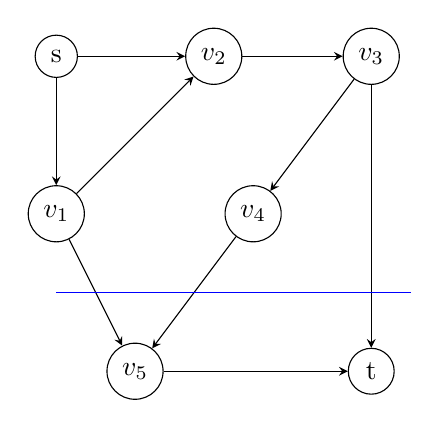
\begin{tikzpicture}[>=stealth, node distance=2cm, every node/.style={draw, circle}]
            % Nodes
            \node[draw] at (0, 0) (s) {s};
            \node[draw] at (0, -2) (v1) {$v_1$};
            \node[draw] at (2, 0) (v2) {$v_2$};
            \node[draw] at (4, 0) (v3) {$v_3$};
            \node[draw] at (2.5, -2) (v4) {$v_4$};
            \node[draw] at (1, -4) (v5) {$v_5$};
            \node[draw] at (4, -4) (t) {t};
    
            % Edges
            \draw[->] (s) -- (v2);
            \draw[->] (s) -- (v1);
            \draw[->] (v1) -- (v2);
            \draw[->] (v1) -- (v5);
            \draw[->] (v2) -- (v3);
            \draw[->] (v3) -- (t);
            \draw[->] (v3) -- (v4);
            \draw[->] (v4) -- (v5);
            \draw[->] (v5) -- (t);

            % Cut
            \draw[blue] (0, -3) -- (4.5, -3);              
        \end{tikzpicture}
    \end{figure}
\end{example}


\begin{theorem}[Max-flow min-cut]
    Given a capacitated network $(V, C)$,
    \[
    \max_{F}\phi_{\text{tot}}(F) = \min_{S}\kappa(S),
    \]
    i.e.,
    the maximum total value over all flows is equal to the minimum cut capacity of the network.
\end{theorem}

\begin{example}
    With these cuts we can see that
    \begin{figure}[H]
        \centering
        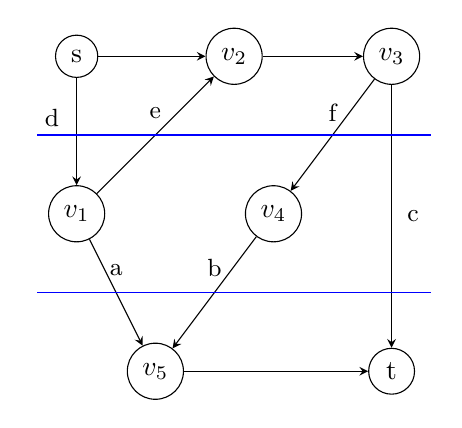
\begin{tikzpicture}[>=stealth, node distance=2cm, every node/.style={draw, circle}]
            % Nodes
            \node[draw] at (0, 0) (s) {s};
            \node[draw] at (0, -2) (v1) {$v_1$};
            \node[draw] at (2, 0) (v2) {$v_2$};
            \node[draw] at (4, 0) (v3) {$v_3$};
            \node[draw] at (2.5, -2) (v4) {$v_4$};
            \node[draw] at (1, -4) (v5) {$v_5$};
            \node[draw] at (4, -4) (t) {t};
    
            % Edges
            \draw[->] (s) -- (v2);
            \draw[->] (s) -- (v1)
                node[midway, left, yshift=5pt, draw=none] {\small d};
            \draw[->] (v1) -- (v2)
                node[midway, above, draw=none] {\small e};
            \draw[->] (v1) -- (v5)
                node[midway, above, draw=none] {\small a};
            \draw[->] (v2) -- (v3);
            \draw[->] (v3) -- (t)
                node[midway, right, draw=none] {\small c};
            \draw[->] (v3) -- (v4)
                node[midway, above, draw=none] {\small f};
            \draw[->] (v4) -- (v5)
                node[midway, above, draw=none] {\small b};
            \draw[->] (v5) -- (t);

            % Cut
            \draw[blue] (-0.5, -3) -- (4.5, -3);
            \draw[blue] (-0.5, -1) -- (4.5, -1);
        \end{tikzpicture}
    \end{figure}
    For the bottom cut we have
    \[
    a + b + c \leq \max{F}
    \]
    and for the top cut we would have
    \[
    d - e + f + c \leq \max{F}.
    \]
    These show how the flow in and out is less than the maximum flow.
\end{example}

\begin{example}
    Construct a maximal flow,
    that is,
    a flow for which $\Phi_{\text{tot}}(F)$ is as big as possible.

    \begin{solution}
        \begin{figure}[H]
            \centering
            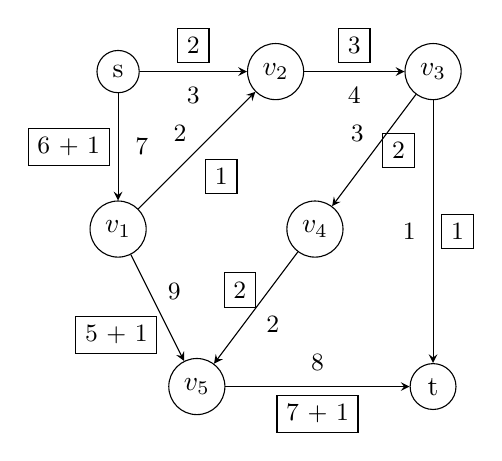
\begin{tikzpicture}[>=stealth, node distance=2cm, every node/.style={draw, circle}]
                % Nodes
                \node[draw] at (0, 0) (s) {s};
                \node[draw] at (0, -2) (v1) {$v_1$};
                \node[draw] at (2, 0) (v2) {$v_2$};
                \node[draw] at (4, 0) (v3) {$v_3$};
                \node[draw] at (2.5, -2) (v4) {$v_4$};
                \node[draw] at (1, -4) (v5) {$v_5$};
                \node[draw] at (4, -4) (t) {t};
        
                % Edges
                \draw[->] (s) -- (v2)
                    node[midway, above, rectangle, yshift = 3pt] {\small 2} 
                    node[midway, below, draw = none] {\small 3};
                    
                \draw[->] (s) -- (v1)
                    node[midway, left, xshift = -3pt, rectangle] {\small 6 + 1}
                    node[midway, right, draw = none] {\small 7};
                    
                \draw[->] (v1) -- (v2)
                    node[midway, below right, rectangle, xshift = 3pt, yshift = -3pt] {\small 1}
                    node[midway, above left, draw = none] {\small 2};
                    
                \draw[->] (v1) -- (v5)
                    node[midway, below left, rectangle, yshift = -3pt] {\small 5 + 1}
                    node[midway, above right, draw = none] {\small 9};
                
                \draw[->] (v2) -- (v3)
                    node[midway, above, rectangle, yshift = 3pt] {\small 3}
                    node[midway, below, draw = none] {\small 4};
                
                \draw[->] (v3) -- (t)
                    node[midway, right, rectangle, xshift = 3pt] {\small 1}
                    node[midway, left, draw = none] {\small 1};
                
                \draw[->] (v3) -- (v4)
                    node[midway, right, rectangle, xshift = 3pt] {\small 2}
                    node[midway, above left, draw = none] {\small 3};
                
                \draw[->] (v4) -- (v5)
                    node[midway, above left, rectangle] {\small 2}
                    node[midway, below right, draw = none] {\small 2};
                
                \draw[->] (v5) -- (t)
                    node[midway, below, rectangle, yshift = -3pt] {\small 7 + 1}
                    node[midway, above, draw = none] {\small 8};
            \end{tikzpicture}
        \end{figure}
        the  minimal cut would be
        \[
        S = \{s, v_1, v_2, v_3, v_4, v_5\}.
        \]
    \end{solution}
\end{example}

For $W \subseteq V$,
define
\[
\phi_{\text{in}}(W) \coloneqq \sum_{u \in V \setminus W}\sum_{v \in W}f_{uv},
\]
the total flow into the set $W$ from vertices outside $W$.
Similarly,
let
\[
\phi_{\text{out}}(W) \coloneqq \sum_{u \in W}\sum_{v \in V \setminus W}f_{uv},
\]
the total flow out of $W$.
With the convention that an empty sum is zero,
note that $\phi_{\text{in}}(V) = \phi_{\text{out}}(V) = 0$
(because there's nowhere outside $V$).

\begin{example}
    Let $W \subset V$ with $y \in V \setminus W$.
    Show that
    \begin{align*}
        \phi_{\text{in}}(W \cup \{y\}) &= \phi_{\text{in}}(W) + \sum_{u \in V \setminus W}f_{uy} - \sum_{v \in W}f_{yv}. \\
        \intertext{Similarly,
        show that}
        \phi_{\text{out}}(W \cup \{y\}) &= \phi_{\text{out}}(W) + \sum_{v \in V \setminus W}f_{yv} - \sum_{u \in W}f_{uy}.
    \end{align*}
    Let $\Delta(W) \coloneqq \phi_{\text{out}}(W) - \phi_{\text{in}}(W)$.

    \begin{solution}
        \begin{align*}
            \phi_{\text{in}}(W \cup \{y\}) &= \phi_{\text{in}}(W) + \phi_{\text{in}}(\{y\}) - \phi_{\text{in}}(W \cap \{y\}) \\
            &= \phi_{\text{in}}(W) + \sum_{u \in V \setminus W}f_{uy} - \text{ flow from $y$ to $W$} \\
            &=\phi_{\text{in}}(W) + \sum_{u \in V \setminus W}f_{uy} - \sum_{v \in W}f_{yv}.
        \end{align*}
        Similarly
        \begin{align*}
            \phi_{\text{out}}(W \cup \{y\}) &= \phi_{\text{out}}(W) + \phi_{\text{out}}(\{y\}) - \phi_{\text{out}}(W \cap \{y\}) \\
            &= \phi_{\text{out}}(W) + \sum_{v \in V \setminus W}f_{yv} - \text{ flow from $W$ to $y$} \\
            &=\phi_{\text{out}}(W) + \sum_{v \in V \setminus W}f_{yv} - \sum_{u \in W}f_{uy}.
        \end{align*}
    \end{solution}
\end{example}

\begin{example}\phantom{}
    \begin{enumerate}[label = (\roman*)]
        \item Show that $\nabla(\{v\}) = 0$ for a single vertex $v \notin \{s, t\}$.

        \item Let $W \subset V$ with $y \in V \setminus W$.
        Use the previous to show that
        \[
        \nabla(W \cup \{y\}) = \nabla(W) + \sum_{v \in V}f_{yv} - \sum_{u \in V}f_{uy}.
        \]

        \item Use induction (i) and (ii) to show that $\nabla(W) = 0$ if $s \notin W$ and $t \notin W$.

        \item Use (ii) and (iii) to show that
        \[
        \nabla(W) = \begin{cases}
            0 & \text{if } s \notin W, t \notin W; \\
            \Phi_{tot}(F) & \text{if } s \in W, t \notin W; \\
            -\Phi_{tot}(F) & \text{if } s \notin W, t \in W; \\
            0 & \text{if } s \in W, t \in W.
        \end{cases}
        \]
    \end{enumerate}

    \begin{solution}\phantom{}
        \begin{enumerate}[label = (\roman*)]
            \item
            From the previous
            \[
            \phi_{in}(W \cup \{y\}) = \phi_{in}(W) + \sum_{u \in V \setminus W}f_{uy} - \sum_{u \in W}f_{yu}
            \]
            \[
            \phi_{out}(W \cup \{y\}) = \phi_{out}(W) + \sum_{u \in V \setminus W}f_{yu} - \sum_{u \in W}f_{uy}.
            \]
            Let $W = \{\}$ any $y = v$.

            \begin{align*}
                \nabla(W \cup \{v\}) &= \phi_{in} - \phi_{out} \\
                &= \phi_{in}(W) + \sum_{u \in V \setminus W}f_{uv} - \left(\sum_{u \in W}f_{vu} + \phi_{out}(W) + \sum_{u \in V \setminus W}f_{vu} - \sum_{u \in W}f_{uv}\right) \\
                \intertext{as $w = \{\}$}
                &= \sum_{u \in V \setminus W}f_{uv} - \sum_{u \in V \setminus W}f_{vu} \\
                &= \sum_{u \in V}f_{uv} - \sum_{u \in V}f_{vu}.
            \end{align*}
            The flow into any vertex is equal to the flow out if it is not $s$ or $t$,
            so
            \[
            \sum_{u \in V}f_{uv} - \sum_{u \in V}f_{vu} = 0
            \]
            such that $v \neq s, t$.

            \item Let $W \subset V$,
            $y \in V \setminus W$.
            \begin{align*}
                \nabla(W \cup \{y\}) &= -\phi_{in} + \phi_{out} \\
                &= -\phi_{in}(W) - \sum_{u \in V \setminus W}f_{uy} + \sum_{u \in W}f_{yu} + \left(\phi_{out}(W) + \sum_{u \in V \setminus W}f_{yu} \cdot \sum_{u \in W}f_{uy}\right) \\
                &= \left(-\phi_{in}(W) + \phi_{out}(W)\right) - \left(\sum_{u \in V \setminus W}f_{uy} + \sum_{u \in W}f_{uy}\right) + \left(\sum_{u \in W}f_{yu} + \sum_{u \in V \setminus W}f_{yu}\right) \\
                &= \nabla(W) - \sum_{u \in V}f_{uy} + \sum_{u \in V}f_{yu}.
            \end{align*}

            \item
            ($1$)
            $w = \{\}, \{v_1\}$,
            $v_1 \neq s, t$.
            ($2$)
            Assume true for $w = \{v_1, \dotsc, v_n\}$,
            $v_i \neq s, t$.
            ($3$)
            $W = \{v_1, \dotsc, v_n\}$ $W = \{v_1, \dotsc, v_n\} \cup \{y\}$ by (ii) $\nabla(W \cup \{y\}) = \nabla W + \sum_{u \in V}f_{yu} - \sum_{u \in V}f_{uy}$,
            by assumption $\nabla W = 0$ and flow into every vertex
            ($\neq s, t$)
            flow out so if $y \neq s, t$ then $\sum_{u \in V}f_{yu} - \sum_{u \in V}f_{uy} = 0$ so $\nabla(W \cup \{y\}) = 0 + 0 = 0$.

            ($4$)
            True for $W = \text{ empty set}$.
            True for $W = \text{ some set $+$ $1$ vertex}$.
            Hence true for all $w$ such that $s, t \notin W$.

            \[
            \nabla(W) = \begin{cases}
                0 & \text{if } s \notin W, t \notin W;\qquad(1) \\
                \Phi_{tot}(F) & \text{if } s \in W, t \notin W;\qquad(2) \\
                -\Phi_{tot}(F) & \text{if } s \notin W, t \in W;\qquad(3) \\
                0 & \text{if } s \in W, t \in W.\qquad(4)
            \end{cases}
            \]
            ($1$) same as (iii)
            ($2$)
            set $y = s$ then $\sum_{u \in V}f_{yu} - \sum_{u \in V}f_{uy} = \Phi_{tot}(F) - 0 = \Phi_{tot}(F)$ as flow out of the source is equal to the total flow,
            so $\nabla(W \cup \{s\}) = \Phi_{tot}(F)$.

            ($4$)
            Take $w_1 = (W \cup \{s\})$,
            $\nabla(W \cup \{s\}) = \Phi_{tot}(F)$,
            take $y = t$
            \[
            \nabla(w_1 \cup \{t\}) = \nabla(w_1) + \sum_{u \in V}f_{tu} - \sum_{u \in V}u_t = \Phi_{tot}(F) + 0 - \Phi_{tot}(F) = 0
            \]
            as flow into sink is equal to the flow out of the source.

            ($3$)
            let $y = t$ then $\nabla(W \cup \{t\}) = o(W) + \sum_{u \in V}f_{tu} - \sum_{u \in V}u_t = 0 + 0 - \Phi_{tot}(F)$ as flow into sink equals total flow so $=\Phi_{tot}(F)$.
        \end{enumerate}
    \end{solution}
\end{example}




\end{document}